\documentclass[11pt]{article}
\usepackage{graphicx}
\usepackage[T1]{fontenc}
\usepackage[polish]{babel}
\usepackage{tabularx}
\usepackage[table,xcdraw]{xcolor}
\usepackage[utf8]{inputenc}
\usepackage{lmodern}
\usepackage{multirow}
\usepackage{array}
\usepackage{booktabs}
\selectlanguage{polish}
\usepackage{titlesec}
\usepackage{amsmath}
\usepackage{esint}
\usepackage{textpos}
\usepackage{chngpage}
\usepackage{calc}
\usepackage{algorithm}
\usepackage[noend]{algpseudocode}
\usepackage{placeins}
\usepackage{longtable}
\usepackage[counterclockwise, figuresleft]{rotating}

\let\Oldsection\section
\renewcommand{\section}{\FloatBarrier\Oldsection}

\let\Oldsubsection\subsection
\renewcommand{\subsection}{\FloatBarrier\Oldsubsection}

\let\Oldsubsubsection\subsubsection
\renewcommand{\subsubsection}{\FloatBarrier\Oldsubsubsection}
\titlelabel{\thetitle.\quad}

\begin{document}
\begin{titlepage}
\centering

{\large Wydział Matematyki i Nauk Informacyjnych Politechniki Warszawskiej}

\vspace{1cm}

\includegraphics[scale=0.15]{logo}
\vspace{3cm}

{\Huge\bfseries Project Game}

\vspace{1cm}

{\Large Sebastian Jakubiak, Mikołaj Karaś, Tomasz Koter}

\vspace{1cm}

{\large v1.0a}

\vspace{1cm}

\vfill

{\itshape {\large 26 listopada 2016r.}}
\end{titlepage}

\tableofcontents


\begin{table}[!h]
\centering
\def\arraystretch{2}%
\caption{Lista zmian}

\resizebox{\textwidth}{!}{
\begin{tabular}{|p{3cm}|p{4cm}|p{6cm}|p{2cm}|}
\hline
Data                 & Autor             & Opis zmiany                                                               & Wersja                                                 \\ \hline
Nov 26, 2016 & Tomasz Koter & Pierwsza wersja dokumentu & 1.0a \\ \hline
                      
\end{tabular}%
}
\end{table}


\newpage

\section{Specyfikacja}

\subsection{Opis biznesowy}
\par
\textit{Project Game} jest grą mającą na celu symulację realizacji pewnego abstrakcyjnego projektu. Grać w nią może w ramach jednej sesji jednocześnie dowolna liczba ludzkich bądź komputerowych graczy w dwóch przeciwnych drużynach, zależna jedynie od upodobań założyciela gry oraz możliwości sprzętowych.
\par
Jako dwie konkurujące drużyny gracze mają za zadanie zrealizować swój projekt jako pierwsi. Drużyna, która jako pierwsza skończy projekt, wygrywa, natomiast ta druga przegrywa.
\par
W ramach jednego projektu wyznaczone są cele, które dana drużyna musi osiągnąć, by zrealizować projekt. Każdy cel osiąga się poprzez podjęcie się zadania i wykonanie go w ramach tego celu. Może się jednak okazać, że wykonane zadanie nijak nie było pomocne w osiągnięciu celu, w związku z czym po wykonaniu go cel pozostaje nieosiągnięty.
\par
Cele i zadania reprezentowane są za pomocą prostokątnej planszy składającej się z kwadratowych pól. Jedno pole może należeć do jednego z trzech obszarów: obszaru zadań, obszaru celów pierwszej drużyny lub obszaru celów drugiej drużyny. Gracze poruszają się po tej planszy w czterech kierunkach, z pola na pole. Zadania generowane są i umieszczane w polach obszaru zadań. Następnie gracze mogą podejmować się tych zadań i wypełniać je poprzez zaniesienie ich z obszaru zadań do obszaru celów swojej drużyny. Gracze nie wiedzą, które pola celów zawierają cel, który przysłuży się zrealizowaniu projektu, a które nie są celem projektu. Odkrywają je dopiero realizując pewne użyteczne zadanie w ramach tego pola. Gracz może upewnić się, czy zadanie jest użyteczne dowiadując się więcej na jego temat, lecz zajmuje to trochę czasu.
\par
Gracze mogą komunikować się między sobą w ramach drużyny i w ten sposób współpracować.

\subsection{Wymagania funkcjonalne}
\par
Poniższy diagram oraz tabela prezentują wszystkie możliwe przypadki użycia systemu gry, co jednocześnie pokrywa postawione w ramach tego projektu wymogi funkcjonalne.

\hspace*{-4cm}
\resizebox{1.5\textwidth}{!}
{
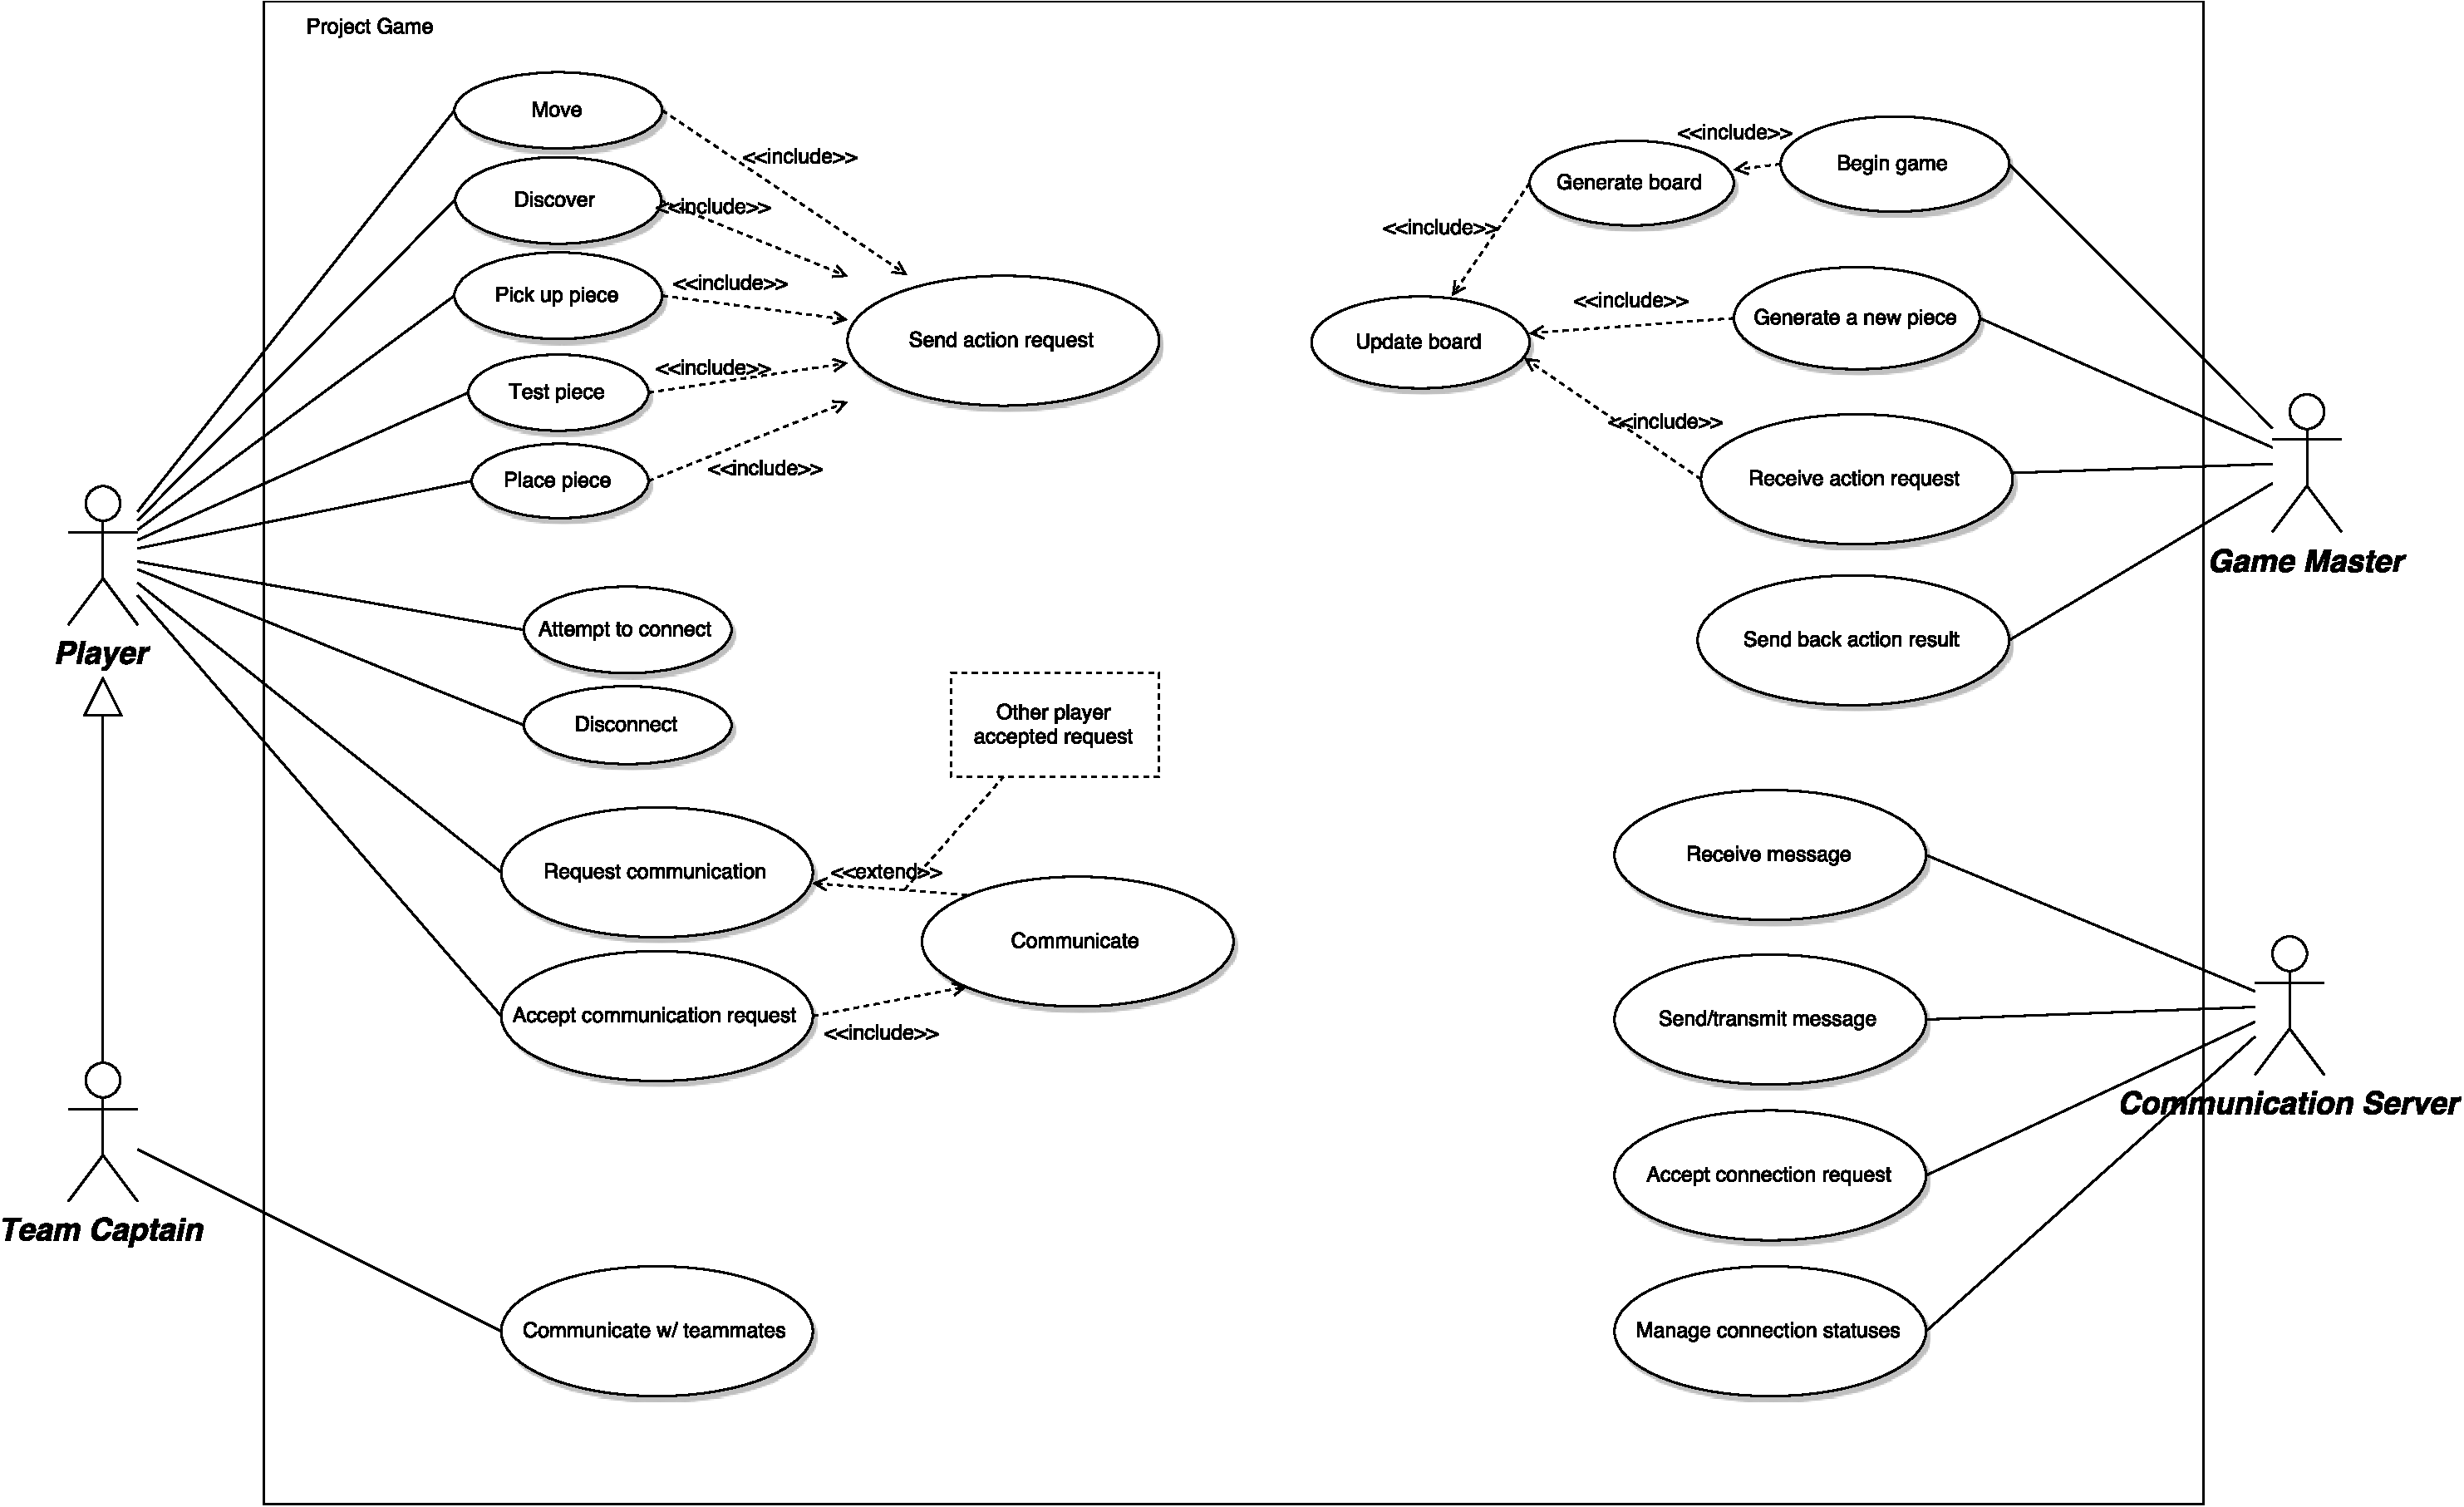
\includegraphics{usecase}
}
\FloatBarrier

\hspace*{-4cm}
\begin{longtable}{|p{.20\textwidth}|p{.03\textwidth}|p{.2\textwidth}|p{.35\textwidth}|p{.35\textwidth}|}
\caption{Przypadki użycia}
\\
\hline
Aktor & Lp & Nazwa & Opis & Odpowiedź systemu \\ \hline
\multirow{11}{.20\textwidth}{Gracz/Kapitan Drużyny} & 1 & Move & Rusz graczem w kierunku góra/dół/lewo/prawo & Gracz zmienia położenie na ekranie lub nie, w zależności od poprawności akcji \\ \cline{2-5}
	& 2 & Discover & Odkryj zawartość otaczających pól oraz poznaj ich odległości od najbliższego zadania & Wypełnia pola w graficznym interfejsie odpowiednimi informacjami \\ \cline{2-5}
	& 3 & Pick up piece & Podnieś zadanie z pola, na którym stoisz & Jeśli gracz stoi na polu z zadaniem, zadanie znika z planszy i jego opis pojawia się w odpowiednim miejscu interfejsu; w przeciwnym przypadku nic się nie dzieje \\ \cline{2-5}
	& 4 & Test piece & Sprawdź, czy zadanie jest użyteczne & Wyświetla się informacja o użyteczności podniesionego zadania. Jeśli jest bezużyteczne, zostaje wyrzucone. \\ \cline{2-5}
	& 5 & Place piece & Użyj zadania do osiągnięcia celu, na którym stoisz & Jeśli zadanie nie było użyteczne, nie dzieje się nic. Jeśli zadanie było użyteczne, odkrywa cel jako osiągnięty i informuje, czy był to cel służący do zrealizowania projektu. \\ \cline{2-5}
	& 6 & Send action request & Wyślij zlecenie wykonania akcji (dowolnego przypadku użycia z przedziału 1-5) przez gracza do Mistrza Gry, by mógł potwierdzić poprawność operacji oraz zaktualizować planszę. Wykonywane bez wywołania przez gracza w momencie zlecenia dowolnej z akcji 1-5 & Aktualizacja planszy widocznej dla gracza i ogólnych informacji o stanie gry \\ \cline{2-5}
	& 7 & Attempt to connect & Spróbuj połączyć się z serwerem gry & Przeniesienie do ekranu lobby w wypadku powodzenia, informacja o błędzie w wypadku niepowodzenia \\ \cline{2-5}
	& 8 & Disconnect & Rozłącz się z serwerem gry (opuść grę) & Przeniesienie do menu głównego gry \\ \cline{2-5}
	& 9 & Request communication & Wyślij do innego gracza prośbę o rozpoczęcie korespondencji & Otwarcie kanału komunikacji między graczami w wypadku zaakceptowania prośby; w przypadku odrzucenia - informacja o tym; w przypadku braku odpowiedzi, po upływie określonego czasu - informacja o tym \\ \cline{2-5}
	& 10 & Accept communication request & Zaakceptuj prośbę komunikacji od innego gracza & Otwarcie kanału komunikacji między graczami. \\ \cline{2-5}
	& 11 & Communicate & Komunikuj się z innym graczem z drużyny. Wyślij/przeczytaj wiadomość od innego gracza. Wymaga zaakceptowania prośby o komunikację przez docelowego członka drużyny (10) & Wyświetlenie wiadomości w okienku czatu \\ \hline
Kapitan Drużyny & 12 & Communicate with teammates & Komunikuj się z innym członkiem drużyny. Kapitan drużyny ma większe kompetencje od zwykłego gracza i nie musi prosić o komunikację. & Wyświetlenie wiadomości w okienku czatu \\ \hline
\end{longtable}
\FloatBarrier

\begin{longtable}[!h]{|p{.20\textwidth}|p{.80\textwidth}|}
\caption{Aktorzy korzystający z systemu}
\\ \hline
Nazwa & Opis \\ \hline
Gracz & Gracz uczestniczący w rozgrywce. Może być człowiekiem lub programem. \\ \hline
Kapitan Drużyny & Wyróżniony gracz, który może bez wysyłania prośby komunikować się z innymi graczami z drużyny. Każda drużyna ma dokładnie jednego kapitana. \\ \hline
\end{longtable}
\FloatBarrier

\subsection{Wymagania niefunkcjonalne}
\par
Żadne wymagania niefunkcjonalne nie zostały określone dla tego projektu.

\subsection{Architektura rozwiązania}
\par
Program zostanie zaimplementowany w strukturze klient-serwer, gdzie klientami będą poszczególni gracze korzystający z aplikacji klienckiej (możliwe będzie korzystanie z jednej maszyny/aplikacji przez kilku graczy jednocześnie z opcją podziału ekranu). Po stronie serwera działać będzie serwer komunikacji oraz jednostka Mistrza Gry.
\par
Wszelka komunikacja gracz-gracz oraz gracz-Mistrz Gry będzie odbywać się za pośrednictwem serwera komunikacji, nawet w wypadku skonfigurowania całego systemu lokalnie na jednej maszynie.

\begin{figure}[!h]
\caption{Architektura systemu}
\resizebox{\textwidth}{!}
{
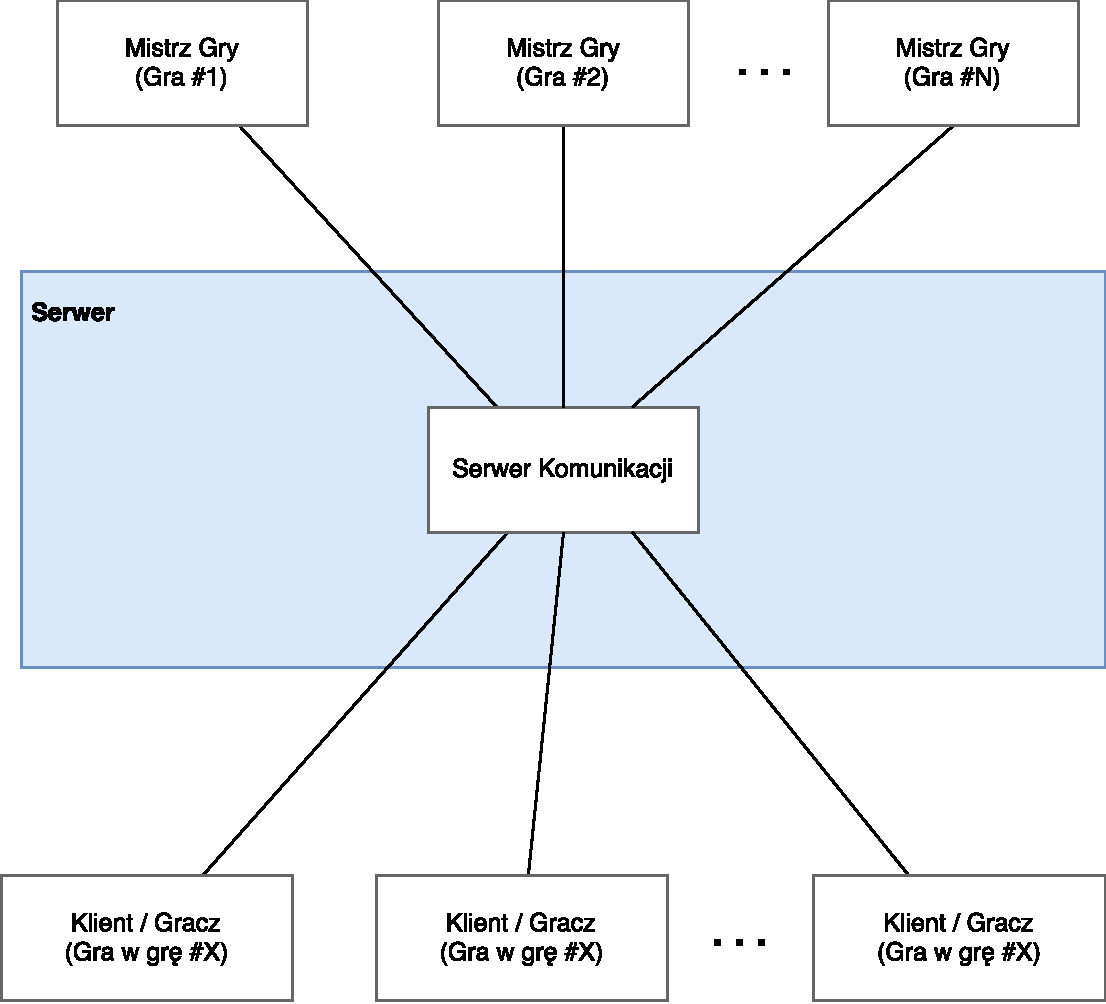
\includegraphics{architecture}
}
\end{figure}
\FloatBarrier

\par
Zależności między obiektami powinny zachodzić jak na poniższym diagramie klas.

\begin{sidewaysfigure}[!h]
\caption{Diagram klas}
\hspace*{-4cm}
\resizebox{1.4\textheight}{!}
{
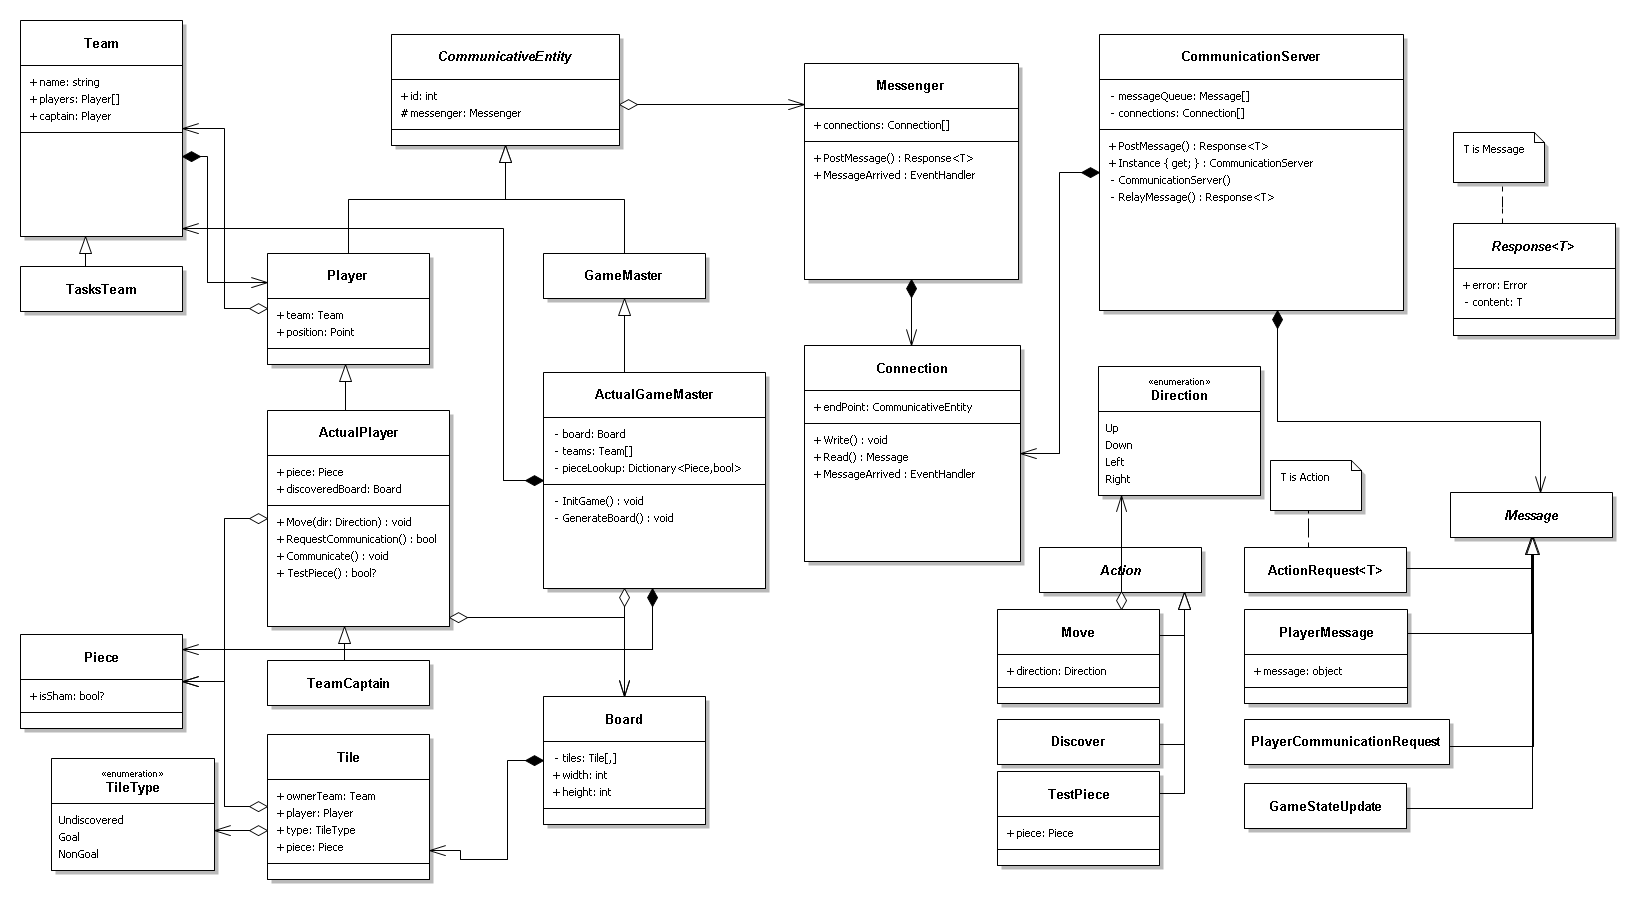
\includegraphics{class_diagram}
}
\end{sidewaysfigure}
\FloatBarrier

\end{document}